%~~~~~~~~~~~~~~~~~~~~~~~~~~~~~~~~~~~~~~~~~~~~~~~~~~~~~~~~~~~~~~~~~~~~~
%    File      : webanalysis
%~~~~~~~~~~~~~~~~~~~~~~~~~~~~~~~~~~~~~~~~~~~~~~~~~~~~~~~~~~~~~~~~~~~~~

\chapter{Introduzione}


Secure Messaging, elaborato del corso di Applicazioni Telematiche, è un'applicazione per la messaggistica sicura, in grado cioè di garantire confidenzialità, integrità e autenticità (mediante protocollo di trasporto DTLS), sviluppata cercando di renderla il più possibile simile ad una reale.
 
L'applicazione è strutturata secondo l'architettura Client/Server: nello specifico il Web Server utilizzato è stato Apache Tomcat, contenente Java Servlet, un modulo NodeJS (con supporto WebSocket) per la gestione della segnalazione  mentre il client è di tipo web, sviluppato facendo uso di HTML, Javascript/JQuery e AJAX, CSS.
Si è inoltre fatto uso di altre tecnologie e linguaggi come ad esempio XACML per il controllo accessi, JSON/XML come formato di interscambio dati (con l'utilizzo delle API JAXB per la manipolazione XML), HTTPS per la comunicazione sicura client/server (sia per il server Tomcat, sia per il server NodeJS), SQL per il database.

Di seguito si definisce e si illustra uno schema di massima astrazione, atto a concepire da un'ottica di alto livello, il funzionamento del sistema.

\begin{figure}[!htbp]
	\centering
	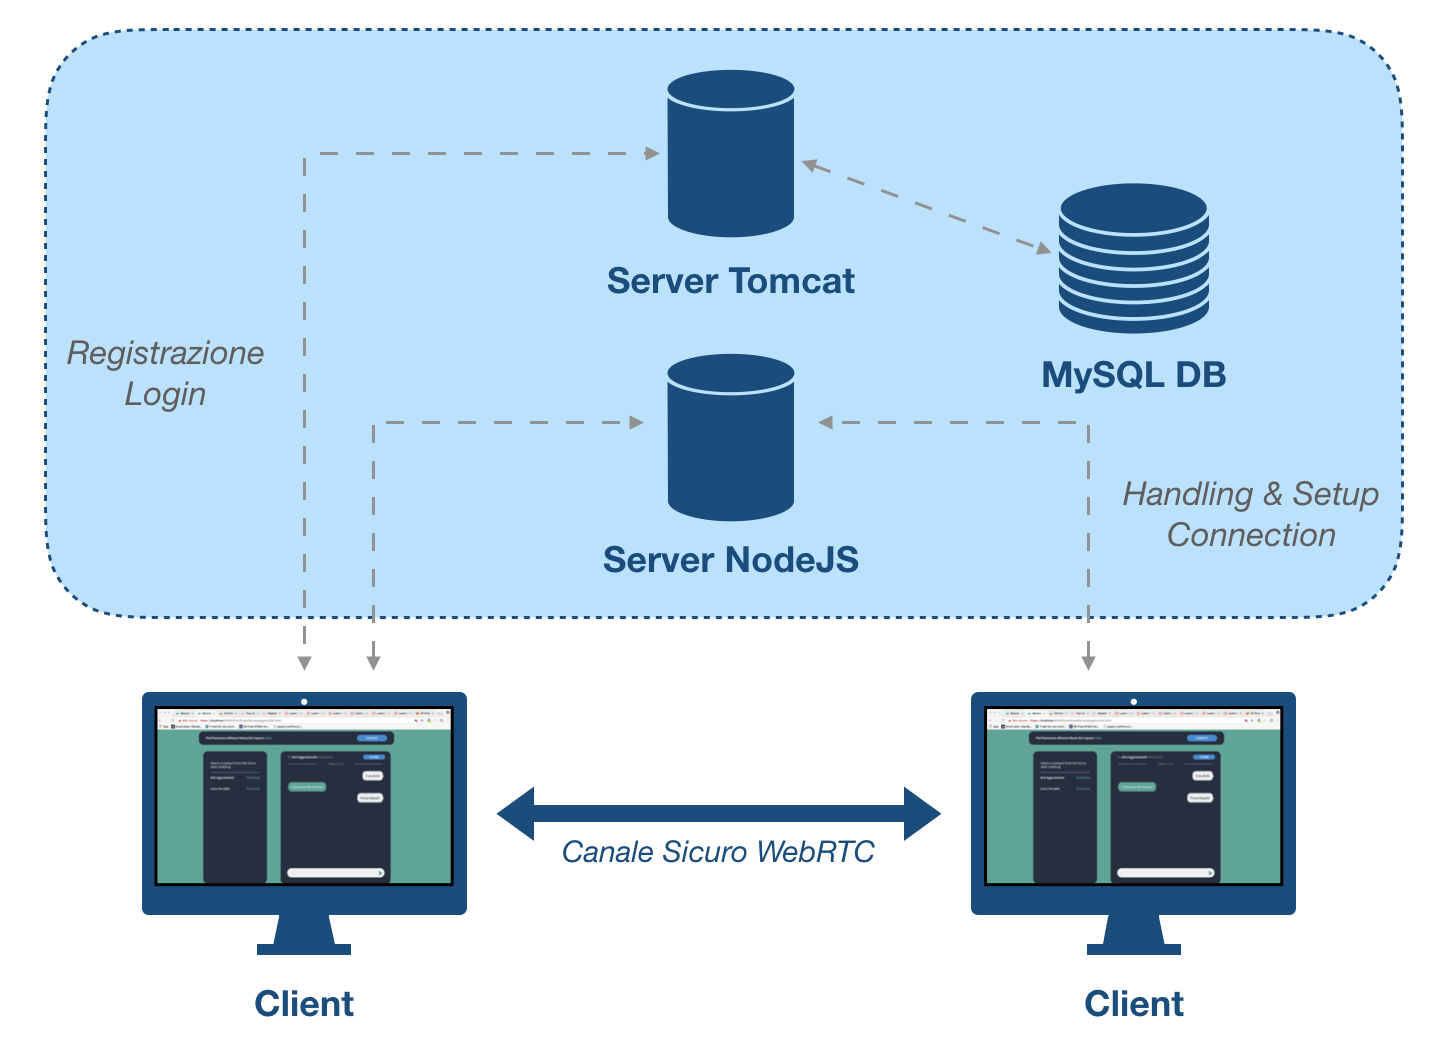
\includegraphics[scale = .6]{img/schemaGenerale}
	\caption{Schema di alto livello dell'applicazione}
	\label{gfx:schemaGenerale}
\end{figure}

Oltre a implementatare la comunicazione crittografata end-to-end facendo uso di WebRTC così come da specifica , sono stati introdotti ulteriori meccanismi che ci aspetteremmo di trovare solo in sistemi effettivamente rilasciati sul mercato: ciò risulta essere il risultato di un percorso di studi che ci ha portato a considerare lo sviluppo di un sistema software o embedded come qualcosa che vada oltre la semplice considerazione di correttezza e prestazioni, ma che include anche altri fattori come robustezza, confidenzialità e integrità.

Tenendo sempre in considerazione i vincoli di tempo e di sviluppatori, sono stati affrontati problemi tipici di applicazioni reali come ad esempio la protezione dell'account, che si è tradotta nella limitazione dei tentativi di accesso all'account (fino al blocco IP) per dispositivo, in modo da frustrare tentativi di attacchi brute-force e autenticazione a due passi. Le password, così come dalle linee guida di numerose organizzazioni, sono state criptate (con salt autogenerato) mediante algoritmo bCrypt. Le richieste contengono token che sono limitati nel numero di utilizzi, caratterizzati da un timestamp (e relativa scadenza), associati ad un IP e firmati dal server per evitare attacchi comuni come il replay attack.\\
Sono state inoltre seguite le direttive \textit{OWASP} per la mitigazione degli attacchi XSS (Cross-Site Scripting) mediante l'utilizzo di \textit{Content Security Policy} (CSP) headers.

Uno sguardo attento è stato rivolto alla considerazione di ogni scenario possibile facendo uso del client web, cercando di garantire che i dati immessi dall'utente siano sempre ben formati alla sorgente (mail, campi numerici, ecc.), garantendo robustezza e alleggerendo il carico del server e riducendo le possibilità di richieste mal costruite ed errori. Un esempio è l'utilizzo di regex per il controllo della validità di una mail.

\newpage